\documentclass[11pt]{article}

\usepackage[T1]{fontenc}
\usepackage[utf8]{inputenc}
\usepackage{newpxtext,newpxmath}
\usepackage[margin=1in]{geometry}
\usepackage{microtype}
\usepackage{amsmath,mathtools}
\usepackage{graphicx}
\usepackage{booktabs}
\usepackage{longtable}
\usepackage{siunitx}
\usepackage{enumitem}
\usepackage{xcolor}
\usepackage{caption}
\usepackage{float}
\usepackage{placeins}
\usepackage[numbers,sort&compress]{natbib}
\usepackage[hidelinks]{hyperref}
\usepackage[nameinlink,noabbrev]{cleveref}
\usepackage{fancyhdr}

\definecolor{cmgnavy}{HTML}{17324D}
\definecolor{cmgblue}{HTML}{2878B5}
\definecolor{cmgteal}{HTML}{2A9D8F}
\definecolor{cmggold}{HTML}{E9A23B}
\definecolor{cmgcoral}{HTML}{E76F51}
\definecolor{cmglight}{HTML}{EEF3F6}

\hypersetup{
  colorlinks=true,
  linkcolor=cmgblue,
  citecolor=cmgteal,
  urlcolor=cmgblue,
  pdftitle={Combinatorial Multigrid, Step by Step},
  pdfauthor={CMG project}
}
\captionsetup{font=small,labelfont=bf}
\sisetup{detect-all,group-separator={,},group-minimum-digits=4}
\setlist{itemsep=0.35em,topsep=0.45em}
\setlength{\parindent}{0pt}
\setlength{\parskip}{0.55em}
\pagestyle{fancy}
\fancyhf{}
\fancyhead[L]{\small Combinatorial Multigrid, Step by Step}
\fancyhead[R]{\small CMG teaching supplement}
\fancyfoot[C]{\thepage}
\renewcommand{\headrulewidth}{0.3pt}

\newcommand{\code}[1]{\texttt{#1}}
\newcommand{\R}{\mathbb{R}}
\newenvironment{takeaway}{\begin{quote}\color{cmgnavy}\textbf{Key idea.}\ }{\end{quote}}
\newenvironment{checkpoint}{\begin{quote}\color{cmgteal}\textbf{Checkpoint.}\ }{\end{quote}}

\newcommand{\ToyVertices}{12}
\newcommand{\ToyEdges}{16}
\newcommand{\ToyLevels}{3}
\newcommand{\ToyTerminal}{Direct}
\newcommand{\ToyIterations}{7}
\newcommand{\ToyRelativeResidual}{\num{6.072e-9}}
\newcommand{\ToyBackwardError}{\num{8.414e-10}}
\newcommand{\ToyMaximumError}{\num{6.988e-9}}

\newcommand{\VenetoRows}{71614}
\newcommand{\VenetoWorkers}{35807}
\newcommand{\VenetoFirms}{5301}
\newcommand{\VenetoMatches}{44050}
\newcommand{\VenetoComponents}{1900}
\newcommand{\VenetoLargestVertices}{34862}
\newcommand{\VenetoLargestWorkers}{31731}
\newcommand{\VenetoLargestFirms}{3131}
\newcommand{\VenetoLargestEdges}{39652}
\newcommand{\VenetoLevels}{3}
\newcommand{\VenetoTerminal}{Direct}
\newcommand{\VenetoIterations}{16}
\newcommand{\VenetoRelativeResidual}{\num{1.840e-6}}
\newcommand{\VenetoBackwardError}{\num{9.322e-9}}
\newcommand{\VenetoMaximumError}{\num{6.977e-3}}
\newcommand{\VenetoRetainedMiB}{\num{1.77}}

\newcommand{\ToyConditionNumber}{\num{61.1}}
\newcommand{\ToyPreconditionedConditionNumber}{\num{2.0}}


\title{\textcolor{cmgnavy}{\Huge Combinatorial Multigrid, Step by Step}\\[0.6em]
\Large A visual and numerical guide to graph-Laplacian solving}
\author{CMG project teaching supplement}
\date{28 August 2026}

\begin{document}
\maketitle

\begin{abstract}
Many large estimation, network, imaging, and simulation problems eventually ask the same numerical question: solve a sparse graph-Laplacian system.  Conjugate gradients (CG) avoids forming a dense inverse, but can still make slow progress when the graph contains weak bridges or widely separated scales.  Preconditioned conjugate gradients (PCG) improves the geometry of the problem.  Combinatorial Multigrid (CMG) supplies the preconditioner by grouping strongly connected vertices, solving related problems on progressively smaller graphs, and lifting the coarse correction back to the original graph.

This supplement develops that sequence from first principles.  A weighted 12-vertex graph makes every hierarchy level and several matrix blocks visible.  A second example is computed from a public Veneto worker--firm teaching extract: it shows an anonymized real graph neighborhood, actual entries of its Laplacian, a materialized block of the CMG action, the complete hierarchy sizes, and certified solve diagnostics.  Every numerical exhibit is generated by the production Rust implementation in this repository.
\end{abstract}

\begin{quote}
\textbf{Origin and attribution.} CMG was introduced by Ioannis Koutis, Gary L. Miller, and David Tolliver in \emph{Combinatorial preconditioners and multilevel solvers for problems in computer vision and image processing} \citep{KoutisMillerTolliver2011}.  Their official MATLAB/C implementation is available in the \href{https://github.com/ikoutis/cmg-solver}{CMG solver repository}; this Rust implementation is developed against \href{https://github.com/ikoutis/cmg-solver/tree/19752fc102f8cae8e34f66457bfaccb1aaa60375}{commit \code{19752fc}} \citep{CmgSolverUpstream}.  The present repository is an independent Rust port, not an official upstream release.
\end{quote}

\tableofcontents
\listoffigures
\clearpage

\section{The problem hiding inside a graph}

\subsection{A network becomes a matrix}

Let a graph have vertices $1,\ldots,n$.  An undirected edge $\{i,j\}$ carries a positive weight $w_{ij}$.  A large weight means that vertices $i$ and $j$ are strongly coupled.  The weighted degree of vertex $i$ is
\[
  d_i=\sum_{j:\{i,j\}\in E} w_{ij}.
\]
The graph Laplacian is the symmetric matrix $L\in\R^{n\times n}$ with
\[
  L_{ii}=d_i,
  \qquad
  L_{ij}=-w_{ij}\quad(i\neq j),
\]
where $L_{ij}=0$ when there is no edge.  Each edge therefore contributes the small block
\[
  w_{ij}
  \begin{bmatrix}
    1 & -1\\[-0.2em]
    -1 & 1
  \end{bmatrix}
\]
to rows and columns $i$ and $j$.

For the weighted path $1\mathrel{-^{2}}2\mathrel{-^{1}}3$, for example,
\[
  L=
  \begin{bmatrix}
    2 & -2 & 0\\
    -2 & 3 & -1\\
    0 & -1 & 1
  \end{bmatrix}.
\]
The diagonal records the total incident weight, while each negative off-diagonal records one link.  Every row sums to zero.

\begin{figure}[htbp]
  \centering
  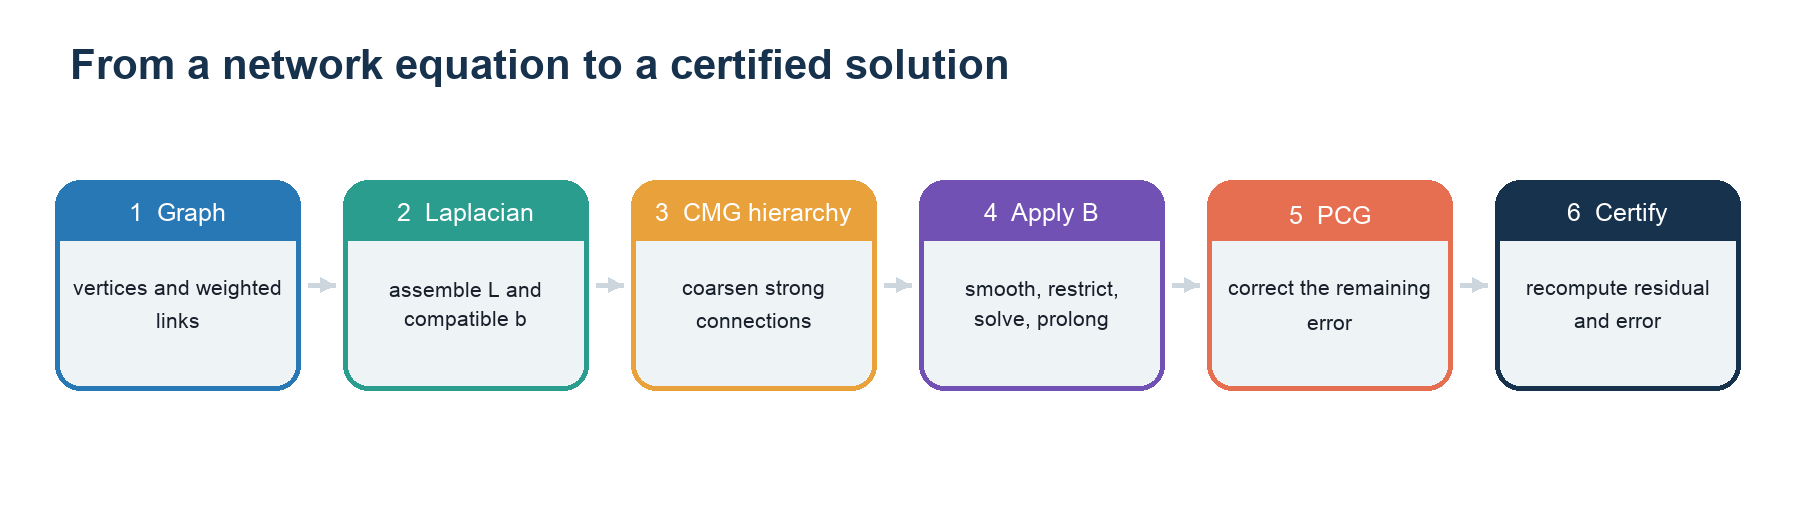
\includegraphics[width=\textwidth]{figures/cmg_pipeline.png}
  \caption{The complete computational story.  CMG is the hierarchy and approximate-inverse stage in the middle; PCG uses it repeatedly, and the final residual is recomputed against the submitted system.}
  \label{fig:pipeline}
\end{figure}

\subsection{Three equivalent ways to read $Lx=b$}

The equation $Lx=b$ can be read in several useful ways.

\begin{enumerate}
  \item \textbf{Balance.} The $i$th equation is
  \[
    (Lx)_i=\sum_j w_{ij}(x_i-x_j)=b_i.
  \]
  Each neighboring difference contributes a weighted flow, and the flows balance the external quantity $b_i$.

  \item \textbf{Energy.} For every vector $x$,
  \[
    x^\top Lx=\sum_{\{i,j\}\in E} w_{ij}(x_i-x_j)^2.
    \tag{1}\label{eq:energy}
  \]
  The energy is small when strongly linked vertices receive similar values.

  \item \textbf{Optimization.} A solution minimizes
  \[
    \phi(x)=\tfrac12 x^\top Lx-b^\top x,
    \tag{2}\label{eq:quadratic}
  \]
  because $\nabla\phi(x)=Lx-b$.
\end{enumerate}

The energy identity also proves that $L$ is positive semidefinite: its quadratic form cannot be negative.  That property is exactly what CG needs, after we handle the null space.

\subsection{Why the Laplacian is singular}

If $\mathbf{1}$ is the all-ones vector, then $L\mathbf{1}=0$.  Adding the same constant to all entries of $x$ leaves every difference $x_i-x_j$ unchanged.  On a connected graph,
\[
  Lx=b \quad\Longrightarrow\quad L(x+c\mathbf{1})=b
\]
for every scalar $c$.  There is a solution only when
\[
  \mathbf{1}^\top b=0.
  \tag{3}\label{eq:compatibility}
\]
For a disconnected graph, the sum must be zero separately within each connected component.  The Rust solver checks this compatibility condition and removes only accepted floating-point drift.  It reports a deterministic component-wise normalization so repeated runs agree.

\begin{takeaway}
The singularity is not a numerical accident.  It expresses a real invariance: only differences are identified.  We solve on the quotient space obtained after ignoring component-wise constants.
\end{takeaway}

\subsection{Why not compute $L^{-1}$?}

First, a Laplacian has no ordinary inverse.  Even after grounding one vertex or imposing a zero-mean restriction, the inverse is usually dense.  Storing a dense $n\times n$ matrix costs $O(n^2)$ memory.  By contrast, a sparse Laplacian stores roughly one diagonal entry per vertex and two matrix entries per edge, and a multiplication $y=Lx$ costs $O(n+m)$ for $m$ edges.

The right strategy is therefore iterative: use only sparse matrix--vector products, vector updates, and a carefully chosen approximate inverse.

\section{Conjugate gradients: solving without an inverse}

\subsection{Residuals are both errors in the equation and directions}

Suppose the current guess is $x_k$.  Its residual is
\[
  r_k=b-Lx_k.
\]
Because $\nabla\phi(x_k)=Lx_k-b=-r_k$, the residual points in the direction of steepest decrease of the quadratic objective introduced above.  Steepest descent would repeatedly move along $r_k$.  On a stretched quadratic bowl it tends to zig-zag.

CG instead constructs search directions $p_k$ that are mutually $L$-conjugate:
\[
  p_i^\top Lp_j=0 \qquad (i\neq j).
\]
Moving along a new direction does not undo the minimization already achieved along earlier directions.  This is the core idea of the method introduced by \citet{HestenesStiefel1952}.

\begin{figure}[htbp]
  \centering
  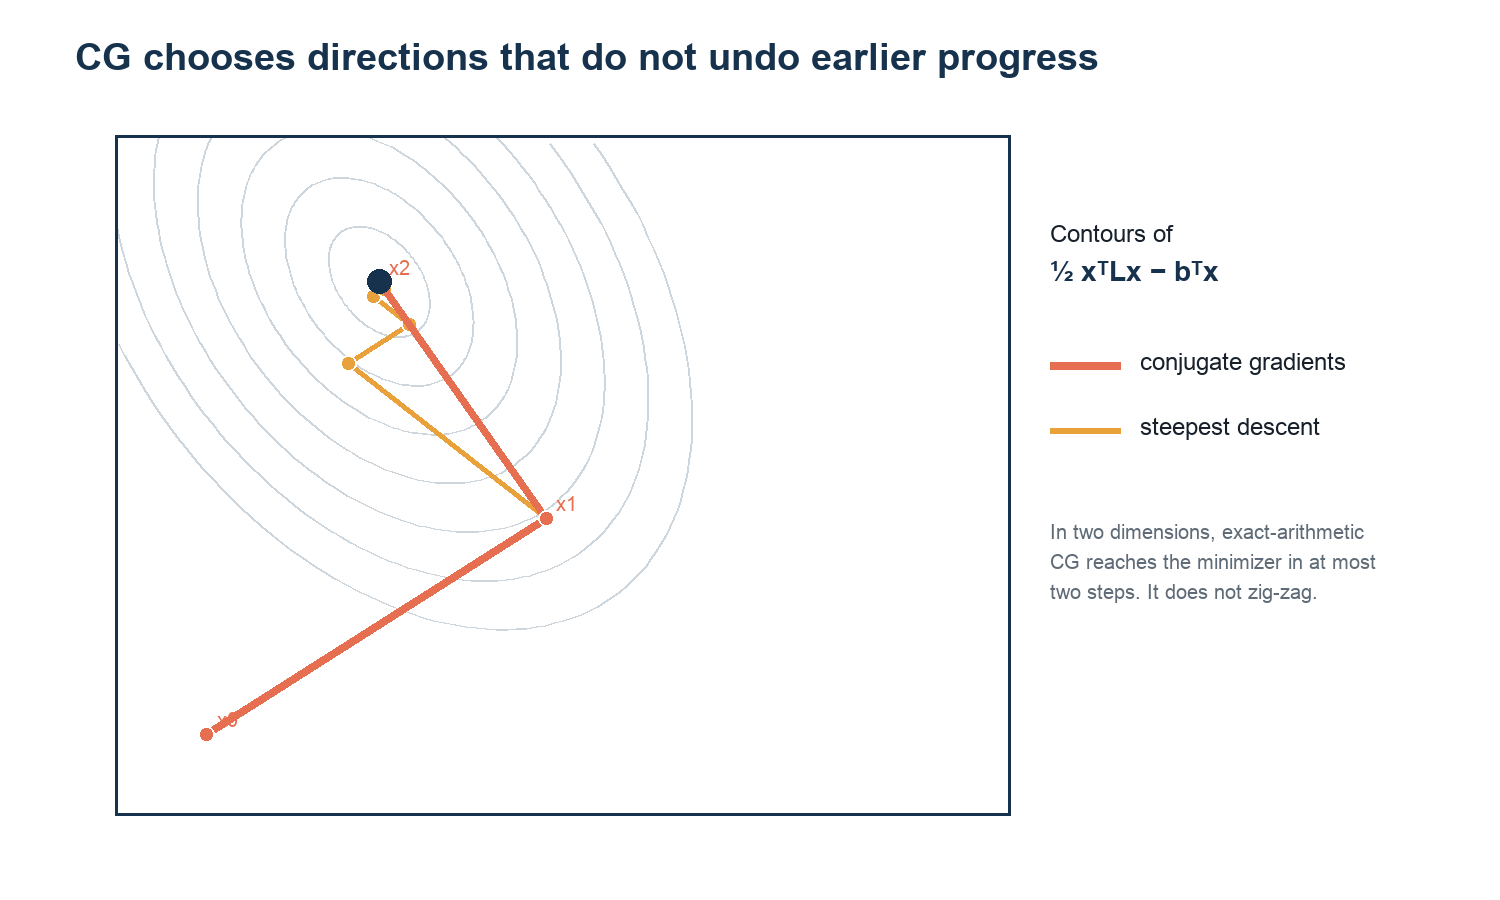
\includegraphics[width=0.92\textwidth]{figures/cg_geometry.png}
  \caption{A two-dimensional quadratic example.  Steepest descent zig-zags across narrow contours.  CG chooses conjugate directions and reaches the exact minimizer in at most two exact-arithmetic steps.}
  \label{fig:cg-geometry}
\end{figure}

\subsection{The CG recurrence}

Starting from $x_0=0$, ordinary CG performs the following operations:
\begin{align*}
  r_0&=b, & p_0&=r_0,\\
  \alpha_k&=\frac{r_k^\top r_k}{p_k^\top Lp_k},
    & x_{k+1}&=x_k+\alpha_kp_k,\\
  r_{k+1}&=r_k-\alpha_kLp_k,
    & \beta_k&=\frac{r_{k+1}^\top r_{k+1}}{r_k^\top r_k},\\
  p_{k+1}&=r_{k+1}+\beta_kp_k.&&
\end{align*}
Only one multiplication by $L$ is needed per iteration.  In exact arithmetic, CG solves an $n$-dimensional positive definite problem within at most $n$ steps.  In practice, rounding error and a large condition number can make many iterations necessary.

For a connected Laplacian, ignore the zero eigenvalue and write the remaining eigenvalues as
\[
  0<\lambda_2\leq\cdots\leq\lambda_n.
\]
The quotient-space condition number is $\kappa(L)=\lambda_n/\lambda_2$.  A small $\lambda_2$ often signals a weak bridge: it is cheap in energy to move one side of the graph relative to the other.  CG then has to resolve both very soft and very stiff directions.

\begin{checkpoint}
If all edge weights are multiplied by ten, $L$ and every nonzero eigenvalue are multiplied by ten, but $\kappa(L)$ is unchanged.  Conditioning is about relative scales, not the overall unit of measurement.
\end{checkpoint}

\subsection{Stopping requires a numerical statement}

A small recursive residual is not enough by itself: accumulated rounding may separate the maintained residual from $b-Lx$.  This crate periodically recomputes the original-system residual and always verifies a convergence candidate.  It reports
\[
  \text{relative residual}=\frac{\lVert b-Lx\rVert_2}{\lVert b\rVert_2}
\]
and the scale-aware backward error
\[
  \eta=\frac{\lVert b-Lx\rVert_2}
  {\lVert b\rVert_2+\lVert L\rVert_{\mathrm{bound}}\lVert x\rVert_2}.
  \tag{4}\label{eq:backward}
\]
The latter asks: relative to the sizes of the submitted data and computed solution, how small a perturbation would make $x$ exact?  A small backward error does not automatically imply a small forward error $\lVert x-x_\star\rVert$ when $L$ is ill-conditioned.

\section{Preconditioned conjugate gradients}

\subsection{Change the geometry, not the answer}

A preconditioner is an operator that is inexpensive to apply and behaves roughly like the inverse of $L$.  It is common to write a positive definite matrix $M\approx L$ and apply $M^{-1}$.  In this supplement we write
\[
  B\approx L^+,
\]
where $B$ denotes the action actually applied to a compatible residual and $L^+$ is the Laplacian pseudoinverse.  The implementation never forms a dense $B$; it evaluates $z=Br$ through a multilevel cycle.

PCG replaces the raw residual direction with the preconditioned residual
\[
  z_k=Br_k.
\]
Its central recurrence is
\begin{align*}
  \alpha_k&=\frac{r_k^\top z_k}{p_k^\top Lp_k},
  &x_{k+1}&=x_k+\alpha_kp_k,\\
  r_{k+1}&=r_k-\alpha_kLp_k,
  &z_{k+1}&=Br_{k+1},\\
  \beta_k&=\frac{r_{k+1}^\top z_{k+1}}{r_k^\top z_k},
  &p_{k+1}&=z_{k+1}+\beta_kp_k.
\end{align*}
The target solution remains $Lx=b$.  The preconditioner changes which error directions are easy for the iteration to remove.

An ideal $B=L^+$ would solve the quotient-space problem in one application.  That would be as expensive as solving the original problem.  A useful preconditioner is deliberately imperfect: applying it must be much cheaper than the iterations it saves.

\section{How CMG constructs the approximate inverse}

\subsection{The multilevel principle}

Ordinary relaxation quickly removes error that changes sharply across adjacent vertices.  It is much slower on smooth error, such as nearly constant values on either side of a weak bridge.  Multigrid represents this smooth error on a smaller graph, where the same large-scale pattern becomes a short-scale pattern that is easier to correct.

CMG makes the smaller graphs using combinatorial information---the weighted connections---rather than a geometric mesh.  The hierarchy is deterministic in this Rust port.

\subsection{Step 1: choose heavy incident connections}

At a level $\ell$, let the graph be $G_\ell$ with Laplacian $L_\ell$.  Each non-isolated vertex selects its maximum-weight incident edge.  Equal-weight ties choose the lower-numbered neighbor.  These selections define a directed parent relation.  Intuitively, a vertex first proposes to stay with the neighbor to which it is most strongly coupled.

The selected relation may contain long or poorly shaped components.  The implementation applies the upstream diameter/conductance forest split, then a low-effective-degree correction.  If the selected tree weight incident to a vertex is too small relative to that vertex's weighted degree, the vertex becomes its own root.  The upstream threshold used here is $1/8$.

\subsection{Step 2: turn forest components into aggregates}

The connected components of the corrected forest are the aggregates.  If fine vertex $i$ belongs to coarse aggregate $a$, define the restriction matrix $R_\ell$ by
\[
  (R_\ell)_{a i}=1,
\]
with all other entries zero.  Restriction sums a fine vector within each aggregate:
\[
  r_c=R_\ell r_f.
\]
Prolongation copies a coarse correction back to each member:
\[
  e_f=R_\ell^\top e_c.
\]

\subsection{Step 3: contract the graph exactly}

The next Laplacian is the Galerkin contraction
\[
  L_{\ell+1}=R_\ell L_\ell R_\ell^\top.
  \tag{5}\label{eq:galerkin}
\]
Edges inside one aggregate disappear; weights of multiple edges between the same two aggregates are summed.  This Galerkin contraction preserves the energy of vectors that are constant within each aggregate:
\[
  y^\top L_{\ell+1}y=(R_\ell^\top y)^\top L_\ell(R_\ell^\top y).
\]
The same construction repeats until a terminal condition is reached.  Production CMG uses a direct grounded LDL factor when a level has fewer than 700 vertices.  Fill growth, weak vertex reduction, full contraction, and a maximum-level guard provide safe alternative stopping conditions.

\subsection{Step 4: apply one stationary CMG cycle}

At a nonterminal level, the smoother uses
\[
  \widetilde D_\ell^{-1}=\operatorname{diag}\left(\frac{1}{2d_i}\right).
\]
Given a compatible right-hand side $r$, one cycle has the following shape:
\begin{enumerate}
  \item form an initial damped-Jacobi approximation $e\leftarrow \widetilde D_\ell^{-1}r$;
  \item compute the remaining residual $s\leftarrow r-L_\ell e$;
  \item restrict and center it, $s_c\leftarrow R_\ell s$;
  \item approximately solve $L_{\ell+1}e_c=s_c$ recursively, using the stored repeat count;
  \item prolong and add, $e\leftarrow e+R_\ell^\top e_c$;
  \item apply a final damped-Jacobi correction.
\end{enumerate}
At a direct terminal, a grounded LDL factor solves the compatible coarse problem.  Repeat counts balance recursive work using nonzero counts and, near a direct terminal, the actual terminal-factor fill.

\begin{takeaway}
Smoothing attacks local, rapidly varying error.  Coarse correction attacks global, slowly varying error.  CMG alternates the two, and PCG corrects whatever the stationary cycle does not remove accurately enough.
\end{takeaway}

\section{A 12-vertex example, all the way down}

\subsection{The graph and its pedagogical setting}

The teaching graph has \ToyVertices\ vertices and \ToyEdges\ weighted edges.  Vertices V1--V6 form one well-connected lobe, V7--V12 form another, and two weak cross-links of weights $0.4$ and $0.25$ connect the lobes.  Within each lobe, the strongest edge has weight $4$, followed by edges of weights $3$, $2$, and smaller links.

The production direct threshold is 700, so a 12-vertex graph would normally go directly to the terminal factor.  To expose the hierarchy, the teaching driver alone sets \code{direct\_threshold = 3}.  No library default or production path is changed.

\begin{figure}[htbp]
  \centering
  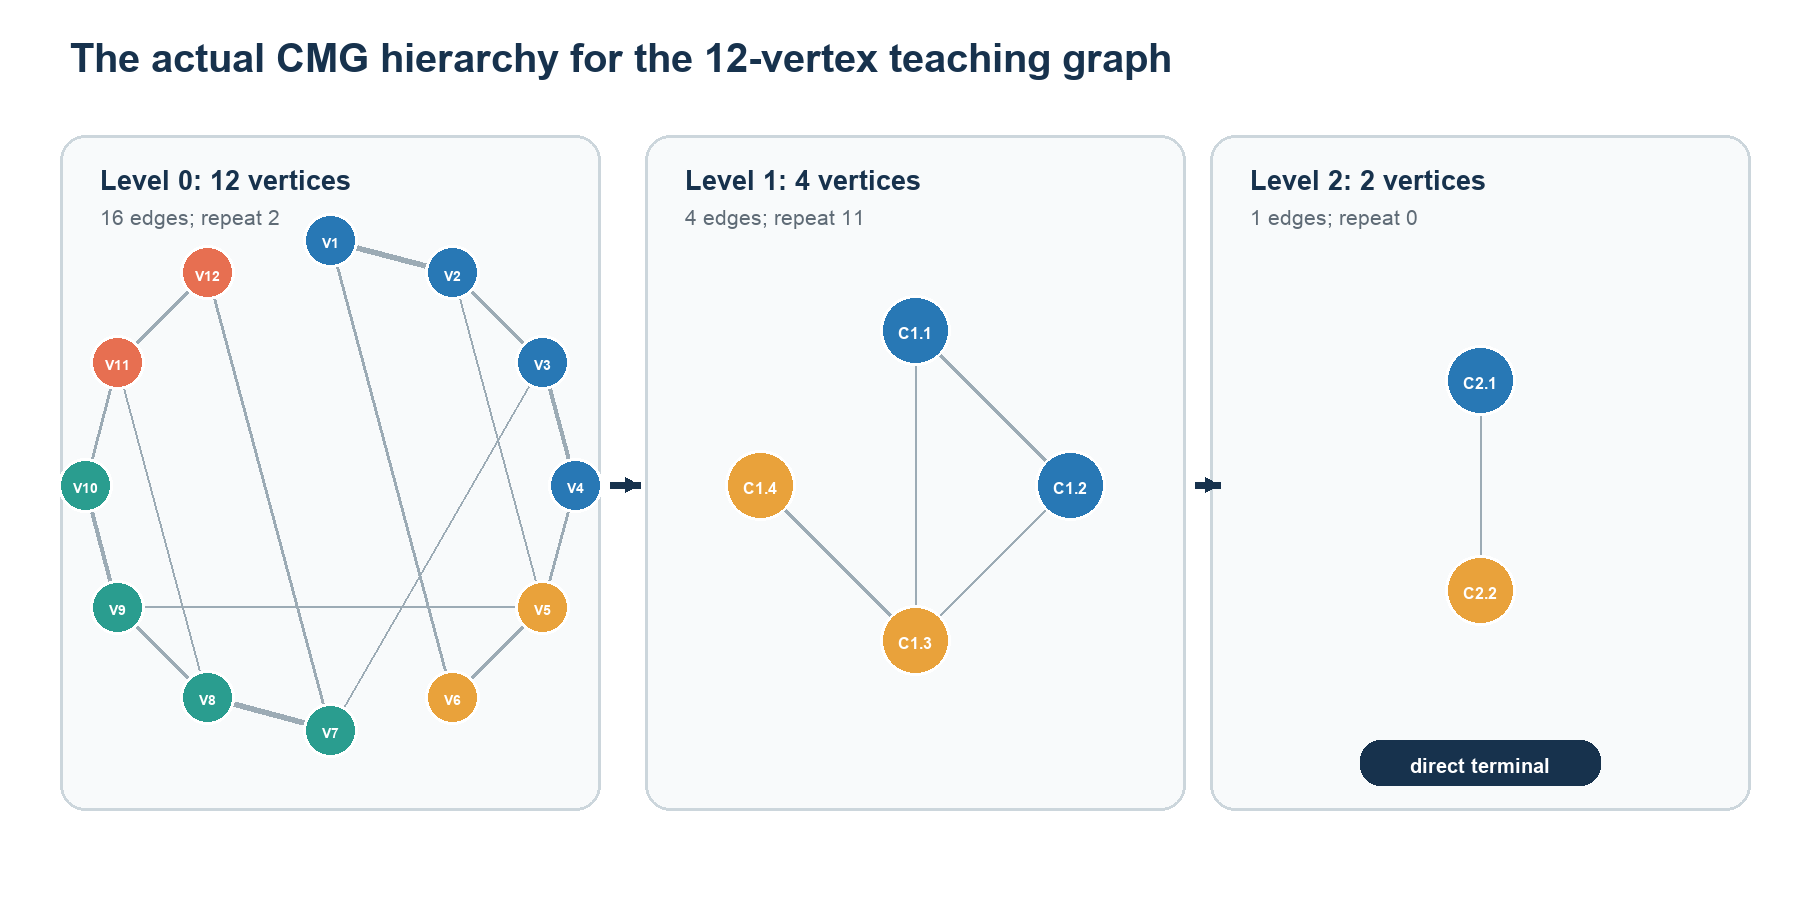
\includegraphics[width=\textwidth]{figures/toy_hierarchy.png}
  \caption{The hierarchy emitted by the Rust implementation.  Colors at a nonterminal level identify vertices that share the same next-level aggregate.  Edge widths reflect weights.}
  \label{fig:toy-hierarchy}
\end{figure}

At level 0, CMG forms four aggregates:
\[
  \{\mathrm{V1,V2,V3,V4}\},\quad
  \{\mathrm{V5,V6}\},\quad
  \{\mathrm{V7,V8,V9,V10}\},\quad
  \{\mathrm{V11,V12}\}.
\]
The resulting four-vertex graph is then grouped into two aggregates, and the two-vertex level is factored directly.  The exact stored hierarchy is:
\begin{center}
\begin{tabular}{rrrrrl}
\toprule
Level & Vertices & Edges & Matrix nnz & Repeat & Terminal \\
\midrule
0 & 12 & 16 & 44 & 2 & --- \\
1 & 4 & 4 & 12 & 11 & --- \\
2 & 2 & 1 & 4 & 0 & Direct \\
\bottomrule
\end{tabular}

\end{center}
The repeat count is not simply the number of coarse vertices.  In particular, the level-1 value of 11 reflects the nonzero balance after the direct terminal factor is known.

\subsection{What the matrices actually look like}

The upper-left $6\times6$ block of the 12-vertex Laplacian is
\begin{center}
\small
\begin{tabular}{lrrrrrr}
\toprule
 & V1 & V2 & V3 & V4 & V5 & V6 \\
\midrule
V1 & 5.20 & -4.00 & 0 & 0 & 0 & -1.20 \\
V2 & -4.00 & 7.80 & -3.00 & 0 & -0.80 & 0 \\
V3 & 0 & -3.00 & 5.40 & -2.00 & 0 & 0 \\
V4 & 0 & 0 & -2.00 & 3.00 & -1.00 & 0 \\
V5 & 0 & -0.80 & 0 & -1.00 & 4.55 & -2.50 \\
V6 & -1.20 & 0 & 0 & 0 & -2.50 & 3.70 \\
\bottomrule
\end{tabular}

\end{center}
Every displayed negative off-diagonal is an edge.  The diagonal of V2 is $4+3+0.8=7.8$, exactly the sum of its incident weights.  The full matrix is sparse.

To make the preconditioner visible, the teaching driver applies CMG to each centered basis vector
\[
  q_j=e_j-\frac{1}{12}\mathbf{1},
\]
centers the returned solution, and places it in column $j$ of a display matrix $B$.  This is a diagnostic materialization of the quotient-space action.  Production code stores the hierarchy and workspaces, not this dense matrix.

The corresponding leading block is
\begin{center}
\small
\begin{tabular}{lrrrrrr}
\toprule
 & V1 & V2 & V3 & V4 & V5 & V6 \\
\midrule
V1 & 0.543 & 0.432 & 0.378 & 0.386 & 0.323 & 0.354 \\
V2 & 0.432 & 0.513 & 0.406 & 0.393 & 0.323 & 0.332 \\
V3 & 0.378 & 0.406 & 0.501 & 0.394 & 0.282 & 0.294 \\
V4 & 0.386 & 0.393 & 0.394 & 0.623 & 0.339 & 0.336 \\
V5 & 0.323 & 0.323 & 0.282 & 0.339 & 0.555 & 0.453 \\
V6 & 0.354 & 0.332 & 0.294 & 0.336 & 0.453 & 0.645 \\
\bottomrule
\end{tabular}

\end{center}
Unlike $L$, $B$ is dense.  A unit imbalance at one vertex produces a response throughout the connected graph.  That global influence is exactly what a useful approximate inverse must capture.

\begin{figure}[htbp]
  \centering
  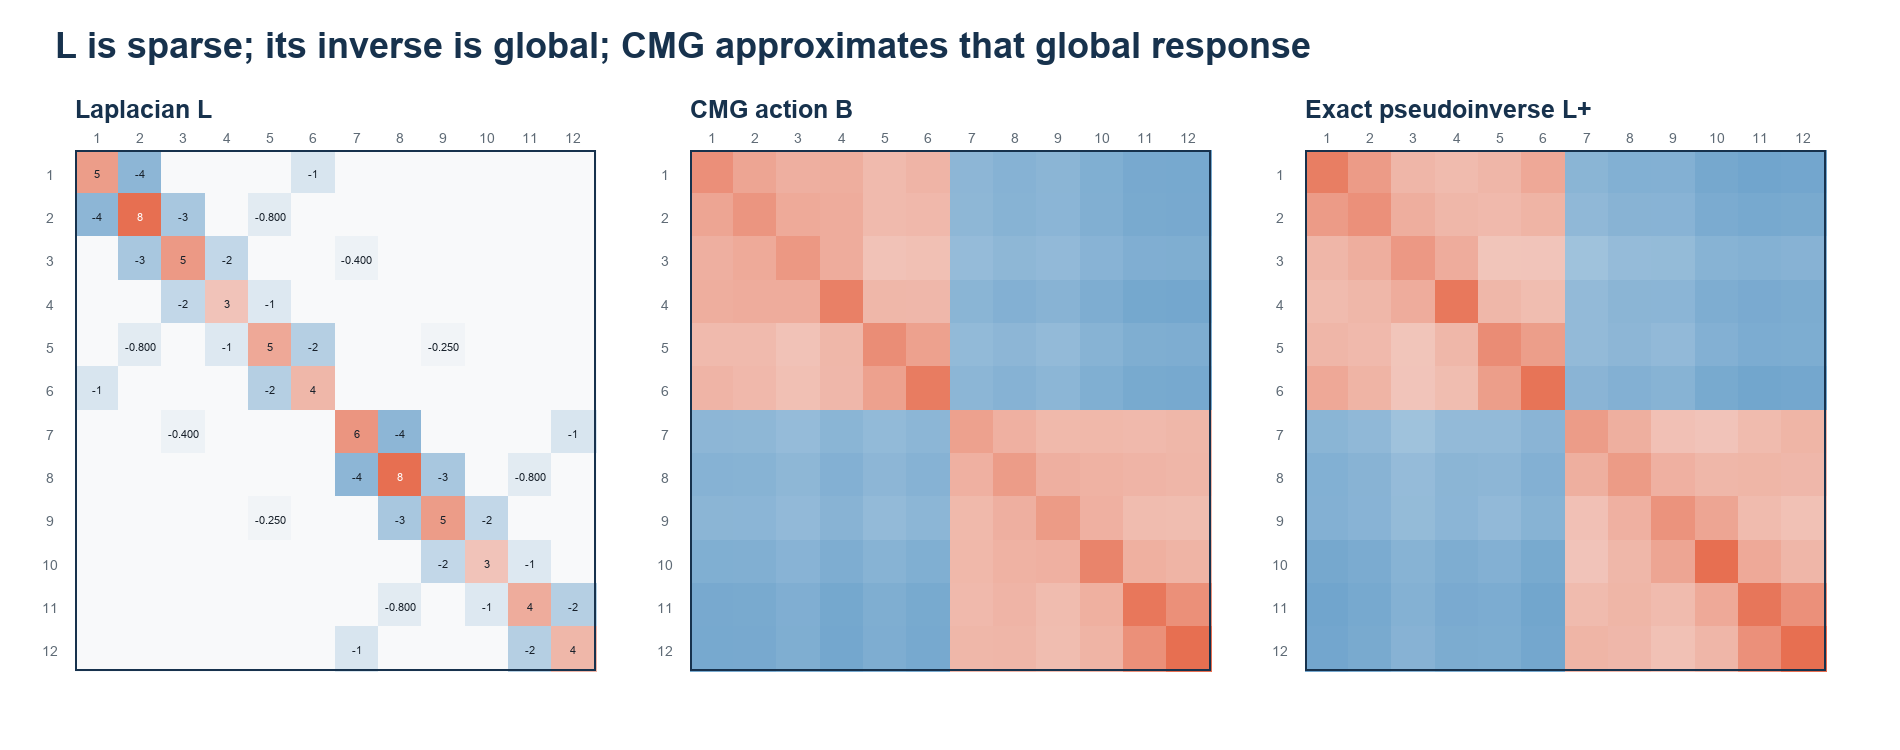
\includegraphics[width=\textwidth]{figures/toy_matrices.png}
  \caption{The full toy Laplacian, the centered CMG action $B$, and the exact pseudoinverse $L^+$.  The two dense response matrices have similar large-scale block structure, although CMG is only approximate.}
  \label{fig:toy-matrices}
\end{figure}

On the zero-mean subspace, the toy Laplacian's spectral condition number is \ToyConditionNumber.  For this diagnostic materialization, the positive eigenvalue spread of $BL$ is about \ToyPreconditionedConditionNumber.  These values explain why the preconditioned iteration sees a much rounder problem.

\subsection{A complete solve}

The driver chooses a deterministic zero-mean vector $x_\star$, constructs $b=Lx_\star$, builds CMG, and runs the production certified PCG solver with its default relative backward tolerance of $10^{-8}$.  It completes in \ToyIterations\ iterations.  The freshly recomputed relative residual is \ToyRelativeResidual, the backward error is \ToyBackwardError, and the maximum coordinate difference from the known zero-mean $x_\star$ is \ToyMaximumError.

\begin{figure}[htbp]
  \centering
  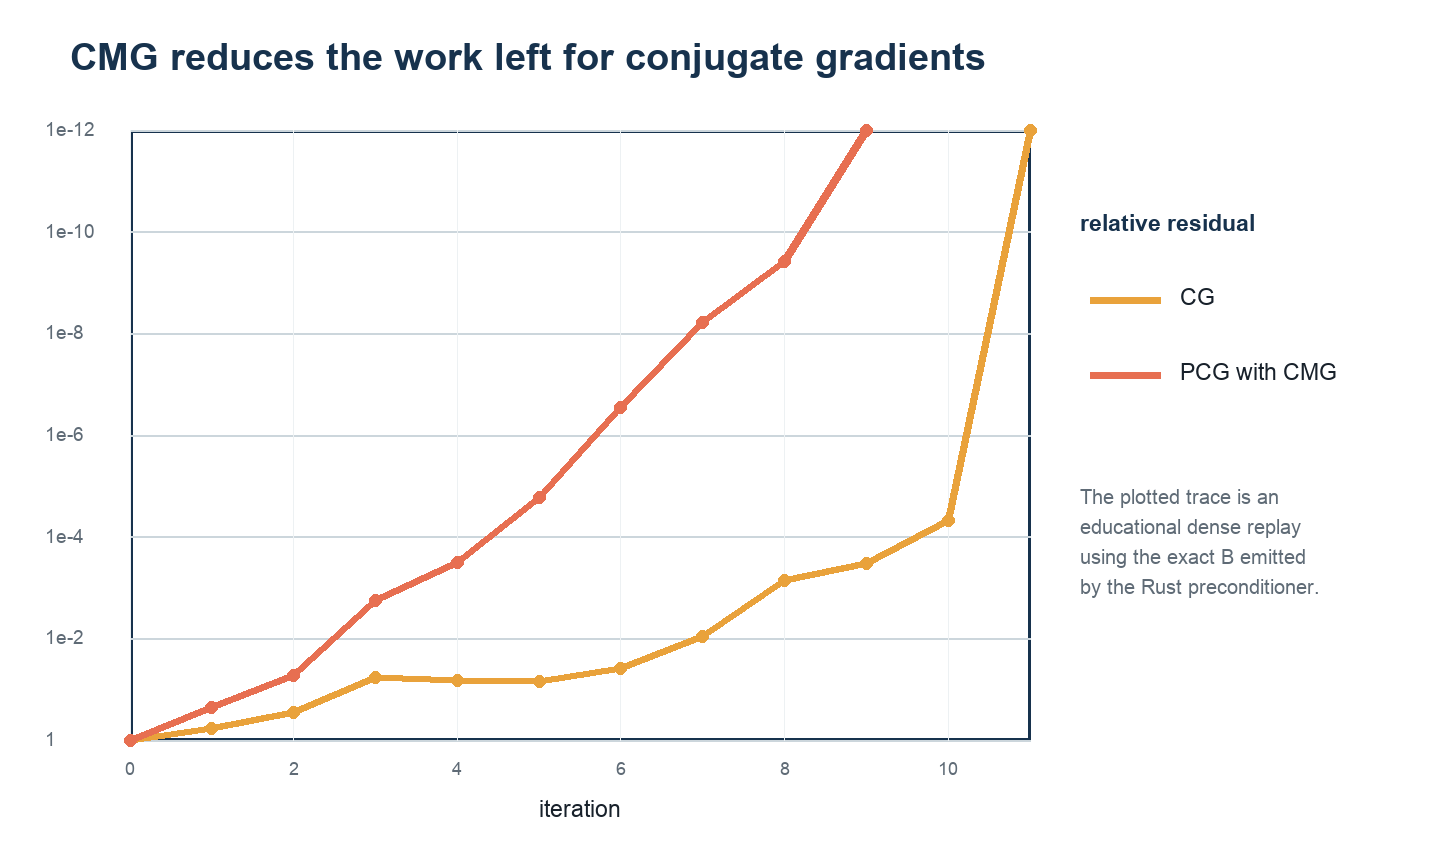
\includegraphics[width=0.92\textwidth]{figures/toy_convergence.png}
  \caption{An educational dense replay of ordinary CG and PCG on the toy system.  The replay uses the exact displayed CMG action $B$; the certified iteration counts above come from the production sparse solver.}
  \label{fig:toy-convergence}
\end{figure}

\FloatBarrier
\section{A real worker--firm graph from the Veneto teaching extract}

\subsection{What the public data are---and are not}

The second example uses \code{inst/extdata/test.csv} from version 0.1.0 of the public CRAN package \code{LeaveOutKSS} \citep{LeaveOutKSS2026}.  Its SHA-256 digest is
\begin{center}
\small\code{93e57a413a8cfccdcb043c5d793105a67b2dc9ebd27d5d3a4f1800abf89a2241}.
\end{center}
It is a public teaching extract associated with a Veneto worker--firm application.  It is \emph{not} the full confidential Veneto Workers History data.  The build checks the digest, keeps source identifiers only in memory, and writes no source worker ID, firm ID, or outcome to the repository.  Displayed nodes receive fresh labels W1, W2, \ldots{} and F1, F2, \ldots{}.

\subsection{Why worker--firm normal equations become a Laplacian}

In the two-way fixed-effects model of \citet{AbowdKramarzMargolis1999}, a simplified observation equation is
\[
  y_{it}=\alpha_i+\psi_{J(i,t)}+\varepsilon_{it}.
\]
Let $D_W$ select the worker and $D_F$ select the firm for each row.  Flip the sign convention of the firm effect and define the incidence matrix
\[
  C=[D_W,-D_F].
\]
Then
\[
  L=C^\top C
\]
is the Laplacian of a bipartite worker--firm graph.  A worker--firm pair observed $w$ times contributes an edge of weight $w$.  Worker and firm diagonals count their weighted observations, while the corresponding off-diagonal is $-w$.

This construction isolates the numerical graph problem.  It does not by itself partial out controls, estimate a complete AKM model, prune leave-out connected sets, or calculate the variance corrections studied by \citet{KlineSaggioSolvsten2020}.  Those tasks are statistical layers around the solver.

\subsection{The graph used here}

The public file has \VenetoRows\ rows, \VenetoWorkers\ distinct workers, \VenetoFirms\ distinct firms, and \VenetoMatches\ distinct worker--firm pairs.  The complete bipartite graph has \VenetoComponents\ connected components.  For a clean single-component numerical illustration, the driver uses the largest component:
\[
  \VenetoLargestVertices\text{ vertices}
  =\VenetoLargestWorkers\text{ workers}
  +\VenetoLargestFirms\text{ firms},
\]
with \VenetoLargestEdges\ canonical weighted edges.

\begin{figure}[htbp]
  \centering
  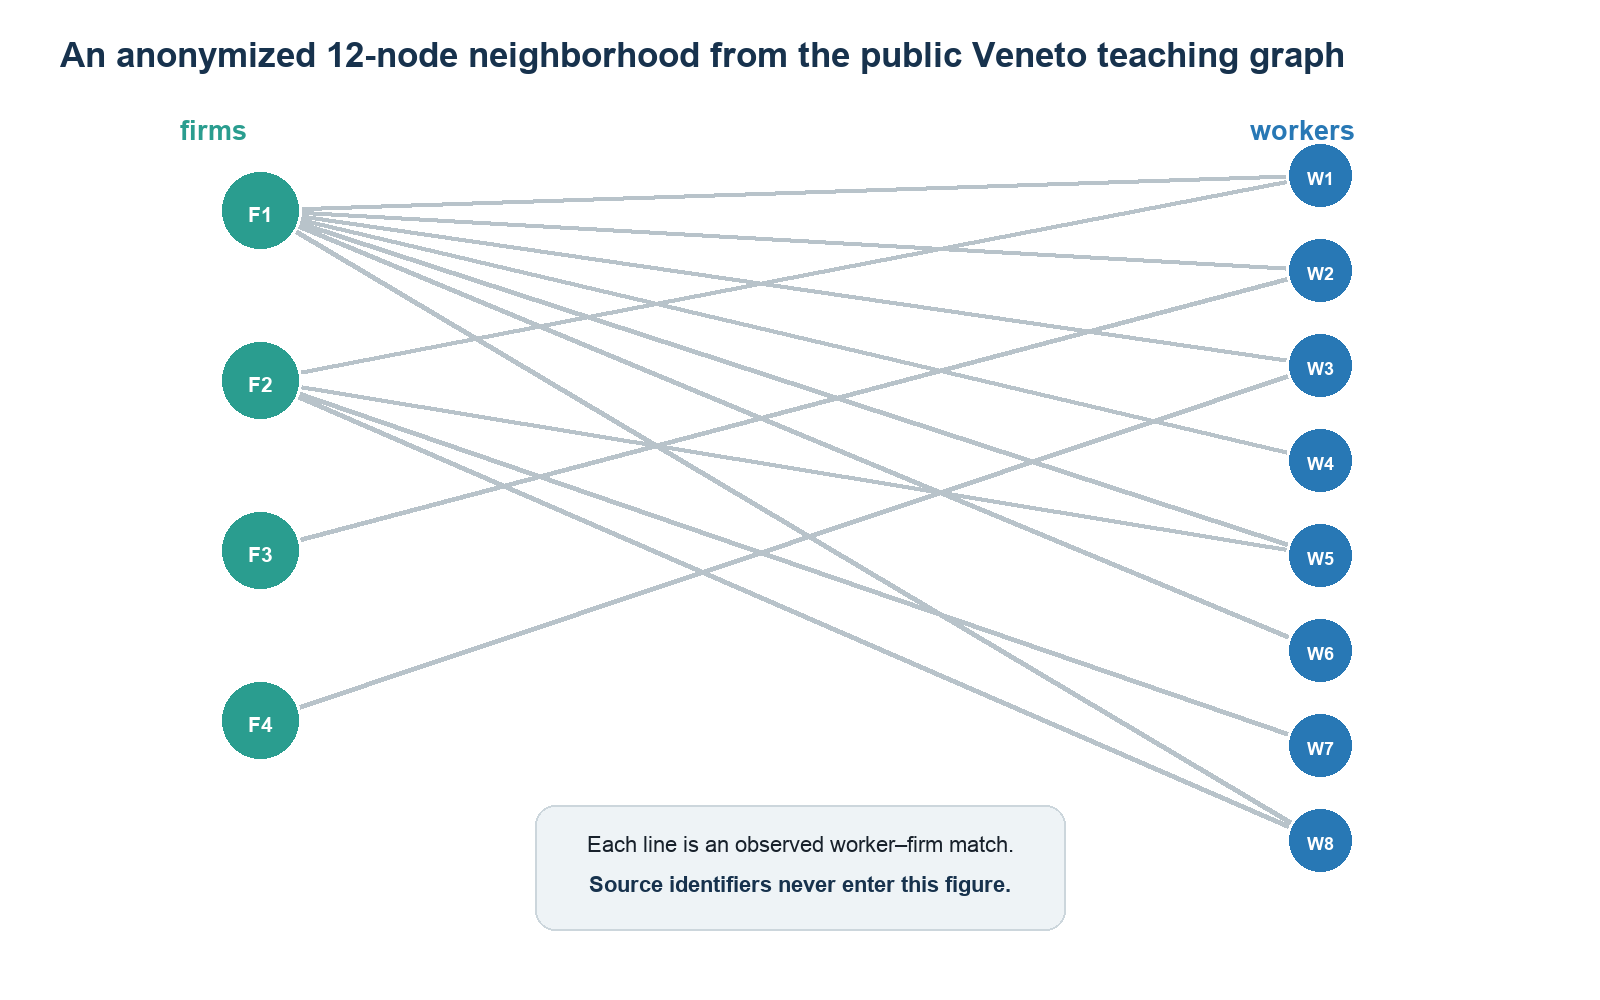
\includegraphics[width=0.94\textwidth]{figures/veneto_neighborhood.png}
  \caption{A deterministic, anonymized 12-node neighborhood selected from the largest connected component.  Mobile workers connect multiple firms and make effects comparable across the mobility graph.}
  \label{fig:veneto-neighborhood}
\end{figure}

\subsection{An actual principal block of $L$}

For the first six displayed nodes, the principal block is
\begin{center}
\small
\begin{tabular}{lrrrrrr}
\toprule
 & F1 & W1 & W2 & W3 & F2 & F3 \\
\midrule
F1 & 7311 & -1 & -1 & -1 & 0 & 0 \\
W1 & -1 & 2 & 0 & 0 & -1 & 0 \\
W2 & -1 & 0 & 2 & 0 & 0 & -1 \\
W3 & -1 & 0 & 0 & 2 & 0 & 0 \\
F2 & 0 & -1 & 0 & 0 & 48 & 0 \\
F3 & 0 & 0 & -1 & 0 & 0 & 636 \\
\bottomrule
\end{tabular}

\end{center}
The entry $L_{\mathrm{F1,F1}}=7311$ is the full weighted degree of F1 in the largest component.  Only some of those neighbors are among the 12 displayed nodes.  Consequently, a principal block of a Laplacian need not have zero row sums: omitted off-block entries still contribute to its diagonal.

\subsection{What the real CMG action looks like}

The next table is a leading block of the centered preconditioner action.  As in the toy example, column $j$ is produced by applying the full, production-built CMG hierarchy to $e_j-\mathbf{1}/n$, centering the result over all $n=\VenetoLargestVertices$ vertices, and selecting the displayed rows.
\begin{center}
\scriptsize
\begin{tabular}{lrrrrrr}
\toprule
 & F1 & W1 & W2 & W3 & F2 & F3 \\
\midrule
F1 & 0.0019 & 0.0017 & 0.0014 & 0.0014 & 0.0014 & 0.0003 \\
W1 & 0.0017 & 0.3804 & 0.0013 & 0.0013 & 0.0172 & 0.0003 \\
W2 & 0.0014 & 0.0013 & 0.3767 & 0.0012 & 0.0011 & 0.0028 \\
W3 & 0.0014 & 0.0013 & 0.0012 & 0.3800 & 0.0011 & 0.0004 \\
F2 & 0.0014 & 0.0172 & 0.0011 & 0.0011 & 0.0633 & 0.0003 \\
F3 & 0.0003 & 0.0003 & 0.0028 & 0.0004 & 0.0003 & 0.0103 \\
\bottomrule
\end{tabular}

\end{center}
The diagonal response for W1 is roughly $0.3804$, but there are nonzero responses at nodes without a direct displayed edge.  The hierarchy has transmitted information through paths elsewhere in the graph.  Again, this dense block is generated only for explanation; the solver applies $B$ without constructing it.

\begin{figure}[htbp]
  \centering
  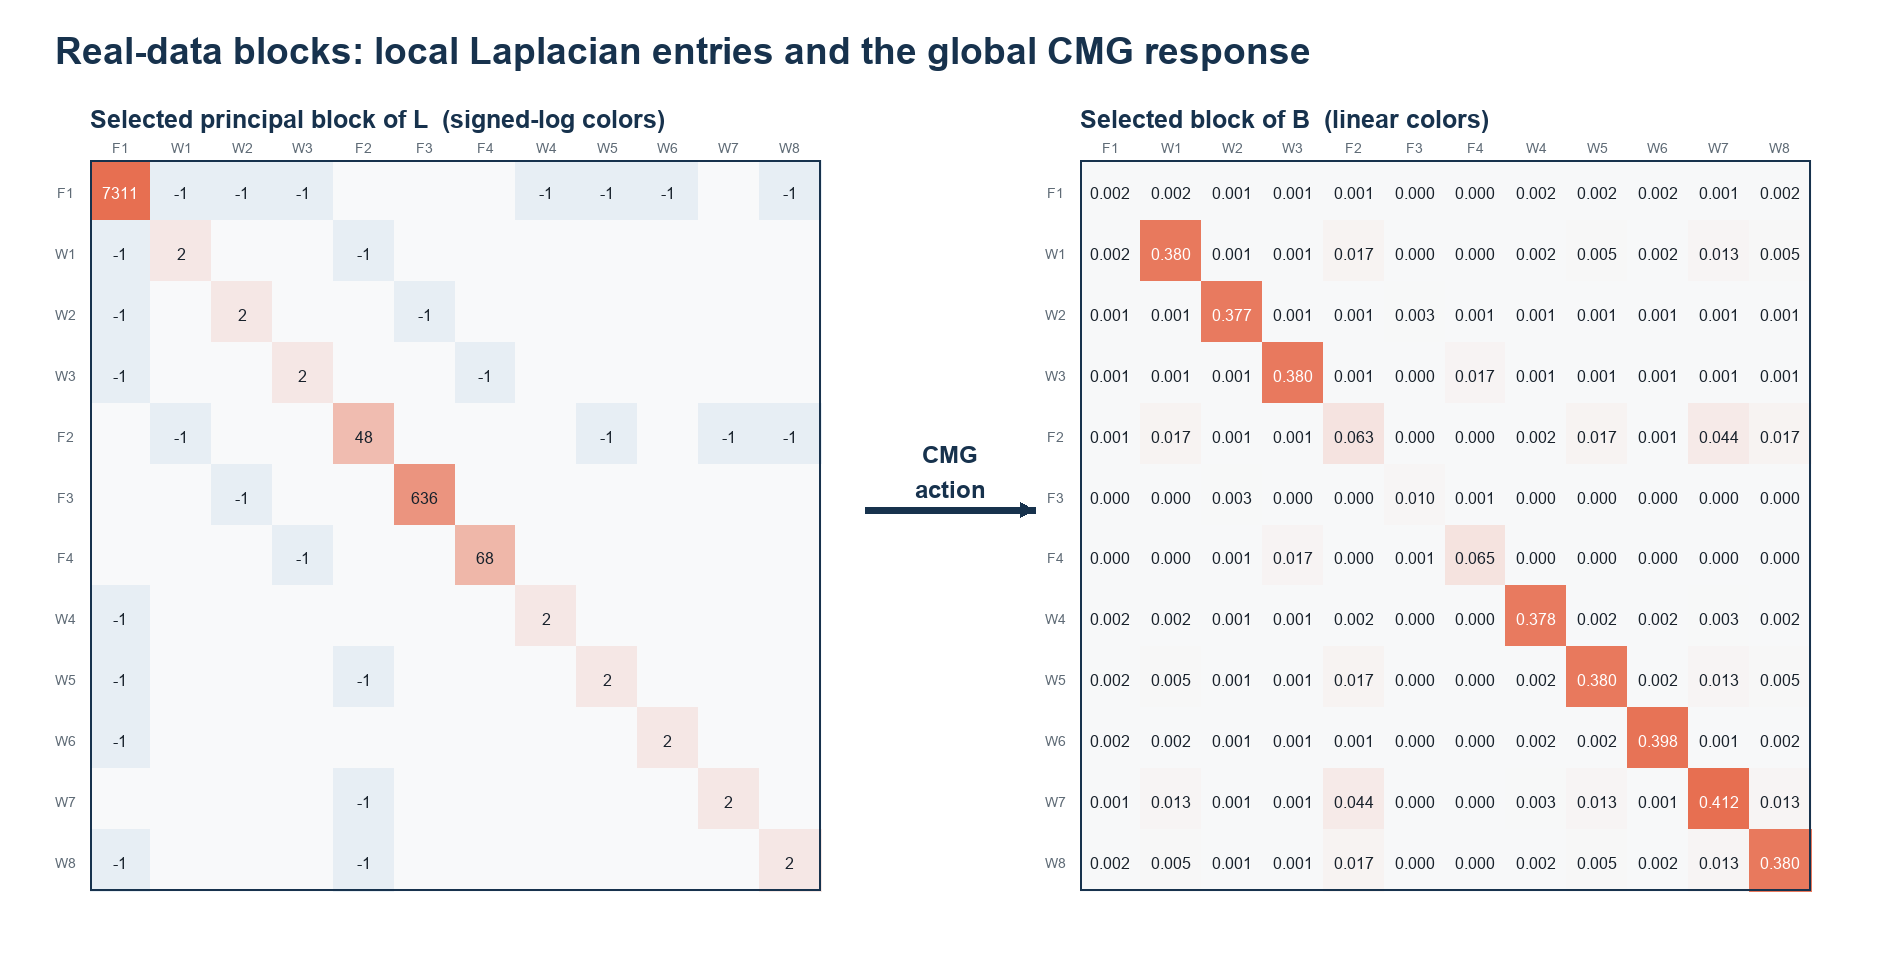
\includegraphics[width=\textwidth]{figures/veneto_blocks.png}
  \caption{Actual entries from the public-data example.  The left panel is a selected principal block of $L$; signed-log colors keep both the $7311$ diagonal and the $-1$ edges visible.  The right panel is the same selected block of the centered CMG action $B$.}
  \label{fig:veneto-blocks}
\end{figure}

\subsection{The complete real-data hierarchy}

Using the production default threshold, CMG builds \VenetoLevels\ levels:
\begin{center}
\begin{tabular}{rrrrrl}
\toprule
Level & Vertices & Edges & Matrix nnz & Repeat & Terminal \\
\midrule
0 & 34,862 & 39,652 & 114,166 & 9 & --- \\
1 & 2,132 & 4,584 & 11,300 & 1 & --- \\
2 & 216 & 1,367 & 2,950 & 0 & Direct \\
\bottomrule
\end{tabular}

\end{center}
The first contraction reduces \VenetoLargestVertices\ vertices to 2,132 aggregates.  The next reduces those to 216 vertices, below the 700-vertex direct threshold.  The complete immutable preconditioner reports \VenetoRetainedMiB\ MiB of principal retained heap storage, including the hierarchy, component metadata, terminal factorization, and repeat counts; allocator bookkeeping is outside that measure.

\begin{figure}[htbp]
  \centering
  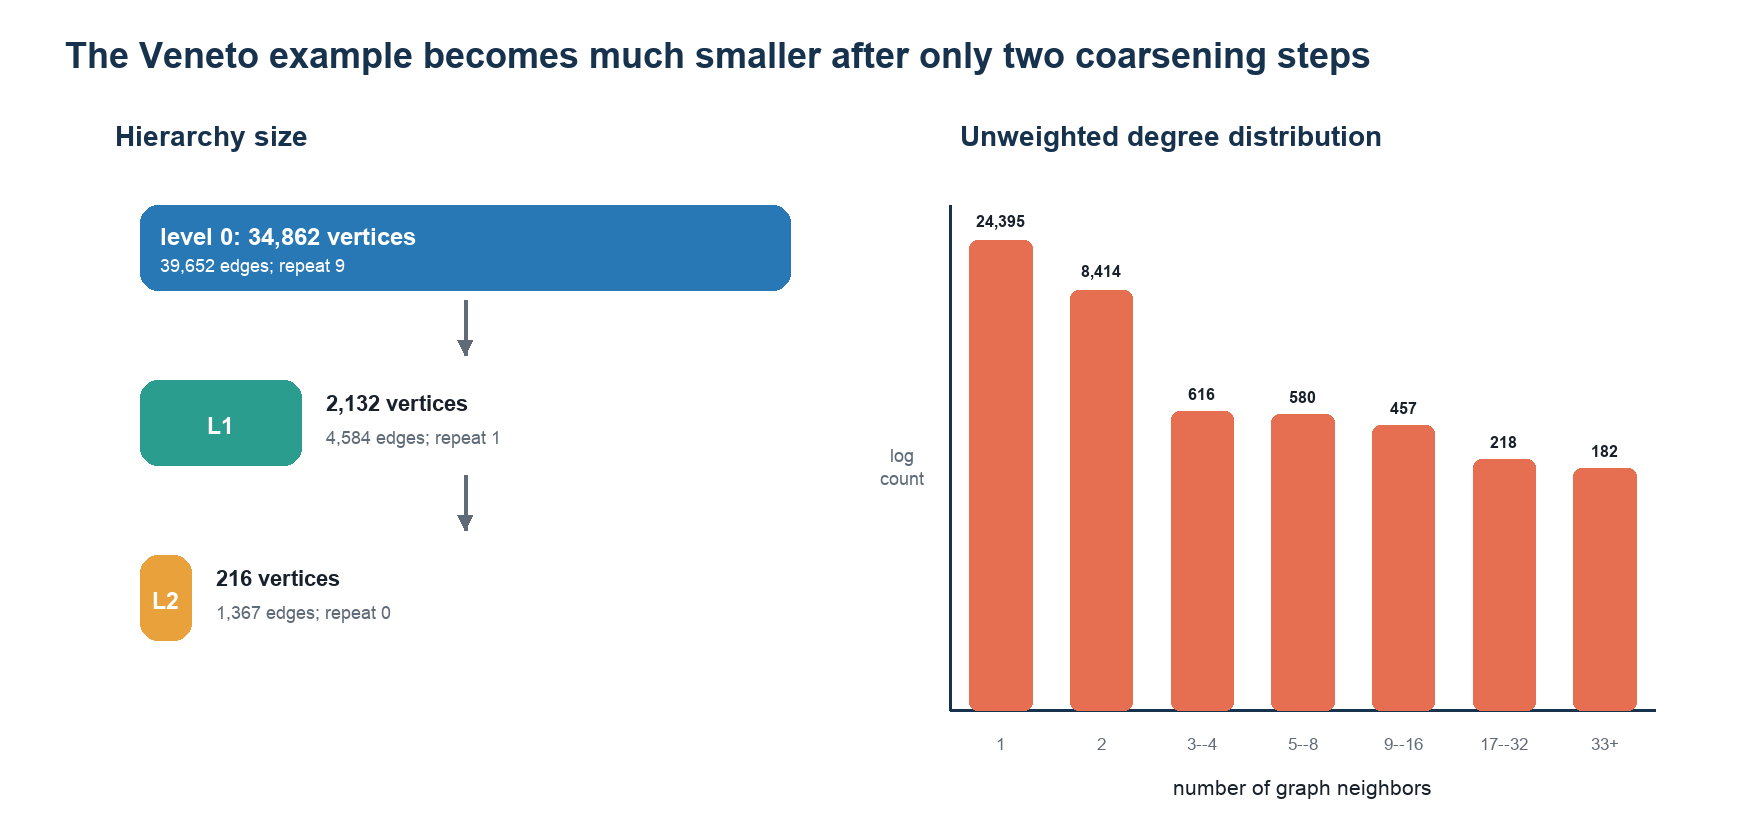
\includegraphics[width=0.98\textwidth]{figures/veneto_hierarchy.png}
  \caption{Left: actual hierarchy sizes.  Right: unweighted degree counts in the largest component; the vertical scale is logarithmic.  Most vertices have one or two graph neighbors, while a smaller set of high-degree firms creates substantial heterogeneity.}
  \label{fig:veneto-hierarchy}
\end{figure}

\subsection{A certified solve and what its diagnostics mean}

The driver constructs a deterministic zero-mean truth $x_\star$, forms $b=Lx_\star$, and solves with the production defaults.  PCG completes in \VenetoIterations\ iterations.  Its recomputed relative residual is \VenetoRelativeResidual, while the certified backward error is \VenetoBackwardError.  The two values differ because the stopping rule uses the scale-aware denominator shown in the stopping criterion; this is expected, and both are reported so the distinction is visible.

The maximum coordinate difference from the known normalized truth is \VenetoMaximumError.  This is much larger than the backward error, illustrating a central numerical lesson: an ill-conditioned system can have a very accurate equation residual while some solution coordinates remain more sensitive.  Statistical applications should choose tolerances with the downstream estimand in mind, not treat one residual number as a universal accuracy guarantee.

\begin{takeaway}
On this real graph, the hierarchy shrinks the problem by more than two orders of magnitude before the direct terminal.  The resulting preconditioner is global even though the original matrix is sparse, and PCG still performs the final accuracy-controlled correction.
\end{takeaway}

\FloatBarrier
\section{Putting the pieces together}

For a new graph-Laplacian solve, the full sequence is:
\begin{enumerate}
  \item \textbf{Assemble and validate.} Canonicalize positive weighted edges, form the diagonal, identify components, and verify that $b$ is component-compatible.
  \item \textbf{Build once.} Construct the heavy-edge forest, forest splits, aggregates, Galerkin coarse graphs, smoothers, repeat counts, and terminal factor.
  \item \textbf{Allocate reusable workspaces.} Keep recursion and PCG vectors out of repeated allocation paths.
  \item \textbf{Apply CMG inside PCG.} Each $z_k=Br_k$ uses the stored stationary cycle.  The graph and hierarchy do not change between iterations.
  \item \textbf{Certify.} Recompute $b-Lx$, report residual and backward error, and retain the component-wise normalization.
  \item \textbf{Reuse when possible.} If edge weights do not change, the same preconditioner and workspace can solve many compatible right-hand sides.  Repeated solves are important in randomized projections, leverage calculations, and leave-out procedures.
\end{enumerate}

\section{Common misconceptions}

\noindent\textbf{``CMG returns the coarse solution.''} No.  Coarse solutions are corrections lifted back to the original graph.  PCG returns a finest-level solution.

\medskip\noindent\textbf{``The preconditioner is a dense stored inverse.''} No.  Dense blocks in this supplement are diagnostic materializations.  Production CMG stores sparse graphs, aggregate maps, diagonal smoothers, a small terminal factor, and workspaces.

\medskip\noindent\textbf{``A small residual means every coordinate is accurate.''} Not necessarily.  Backward accuracy and forward accuracy differ, especially for ill-conditioned graphs.

\medskip\noindent\textbf{``More levels are always better.''} No.  Coarsening must save more work than recursion costs.  CMG uses fill and stagnation guards as well as a direct threshold.

\medskip\noindent\textbf{``Any symmetric matrix is a graph Laplacian.''} No.  A graph Laplacian has nonpositive off-diagonals, zero row sums, and nonnegative edge weights.  The crate also supports SDDM systems through its documented augmentation, but not arbitrary indefinite or nonsymmetric matrices.

\section{Exercises for checking understanding}

\begin{enumerate}
  \item For the three-vertex example in Section 1, verify the energy identity by multiplying out $x^\top Lx$.
  \item Explain why $b=(1,0,0)^\top$ is incompatible on a connected three-vertex graph.  Construct the closest vector obtained by subtracting its mean.
  \item In the toy hierarchy, write the $4\times12$ restriction matrix $R_0$ from the four displayed aggregates.  What does $R_0r$ do to a residual vector?
  \item Why can the displayed Veneto principal block have a diagonal of 7311 but only seven visible $-1$ entries in that row?
  \item Suppose an application solves 1,000 right-hand sides on an unchanged graph.  Which costs can be amortized, and which operations must still occur for every right-hand side?
  \item A run has backward error $10^{-9}$ but a forward error of $10^{-3}$.  Give a graph feature that can make both statements true.
\end{enumerate}

\section{Reproducing every exhibit}

The numerical CSV files, compact tables, and figures are generated from the production crate by the benchmark-only binary \code{teaching-supplement}.  The raw Veneto file is not copied into this repository.  From the repository root, run
\begin{verbatim}
docs/teaching/build.sh /absolute/path/to/kss_example_1999_2001.csv
\end{verbatim}
The script verifies the SHA-256 digest, runs the Rust exporter, regenerates figures and tables, compiles this document with TeX Live, checks the LaTeX log, and creates a standalone HTML translation with embedded images.  Detailed prerequisites and output paths are in \code{docs/teaching/README.md}.

\appendix
\section{Notation at a glance}

\begin{longtable}{ll}
\toprule
Symbol & Meaning\\
\midrule
$G=(V,E,w)$ & Undirected graph with positive edge weights\\
$L$ & Weighted graph Laplacian\\
$d_i$ & Weighted degree of vertex $i$\\
$b$ & Compatible right-hand side\\
$x$ & Solution, defined up to component-wise constants\\
$r=b-Lx$ & Residual\\
$R_\ell$ & Fine-to-coarse restriction at hierarchy level $\ell$\\
$R_\ell^\top$ & Coarse-to-fine prolongation\\
$B$ & Stationary CMG approximate-inverse action\\
$L^+$ & Exact Moore--Penrose pseudoinverse\\
$\eta$ & Reported backward error\\
\bottomrule
\end{longtable}

\section{Scope of the numerical exhibits}

The 12-vertex threshold override exists only to reveal internal levels.  The Veneto example uses the public extract's largest connected component and unit-or-count match weights; it is a solver illustration, not a reproduced empirical estimate.  The selected dense blocks depend on the displayed normalization and are not data structures retained by the production solver.  All dimensions, hierarchy levels, matrix entries, repeat counts, memory values, and solve diagnostics in this document were regenerated from the current source at build time.

{\small
\setlength{\bibsep}{0.25em}
\bibliographystyle{plainnat}
\bibliography{references}
}

\end{document}
